\section{Classification}

\subsection{URL Classification}

Recent studies on malware detection appears to show the idea of applying classification algorithm has became more popular. The classifier applied tries to separate the malicious data from the clean data. Therefore, in all cases a binary classifier has been used. One of the requirements when designing a classifier for the detection system is to have a dataset in advance. The dataset is used as an input for the classifier. Therefore, having a classifier saves resources and makes the system more efficient and robust.Research has been performed to design a system to detect a malicious dynamic HTML code with the aid of a variant classification algorithm. The researchers compared the performance of their system with some anti virus software. The result of their comparison indicates the tolerance of anti virus software is between 40\% and 80\%. This observation shows the lack of intelligent malware detection system that detects any type of attack. Most anti virus software used signature-based technique for malware detection\cite{Macilious-weblearning}  
 The following section describes the details of the classification algorithm employed for this project. 
\subsubsection{Design}
The classification algorithm is made up of two main units, the URLs database and the classifier unit. Figure \ref{fig:clas-1} demonstrates the architecture of the classification module.

\begin{figure}[htb]
\centering
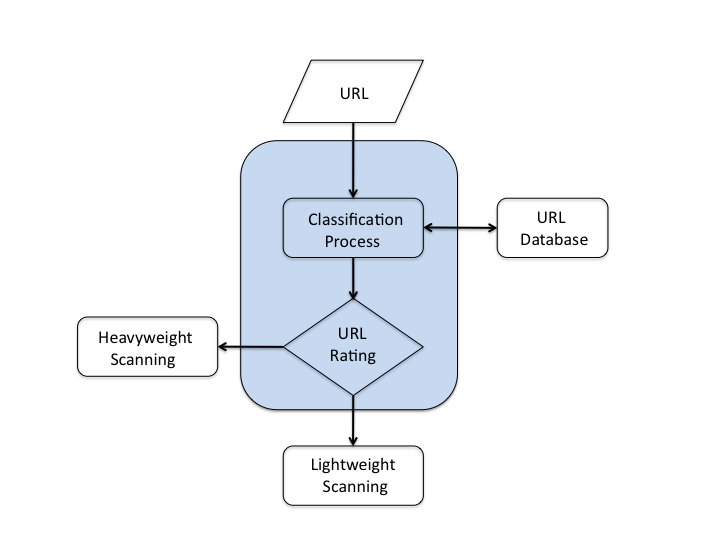
\includegraphics[width=0.8\textwidth]{img/classification(diag).png}
\caption{Classification module architecture}
\label{fig:clas-1}
\end{figure}

% inserted the image of the flowchart for the classification algorithm


\paragraph{} 
The URLs database contains a list of URLs that specifies whether that URL is malicious or not. The URLs database will receive feeds from five different sources, being five different malware detection systems.The second component of the classification algorithm is the classifier unit. A new URL first enters the classifier unit and the classifier checks the structure of the new URL against the structure of URLs listed in the database. Based on the classifier algorithm decision, there will be three outcomes for the maliciousness of the new URL. If the new URL already exists in the database the classifier will immediately confirm whether or not the URL is malicious and hence there is no need to perform more scanning on that URL. However, if the URL does not exist in the database and the classifier returns a poor confidence rate then the new URL needs to be subjected to the heavyweight scanning process. Otherwise, the URL will follow the lightweight scanning process. Section 2 explains the implementation of the classification algorithms in more detail

